\subsubsection{Example}

    \begin{itemize}[noitemsep,topsep=0pt]
      \item Starting position: (32.0, -43.0, 93.0)
      \item End position: (-18.0, -16.0, 8.0) 
      \item Euclidean distance from the object: 25.37715508089904
      \item Object can be seen: False
      \item Success: False
      \item Object type: a black truck
      
    \end{itemize}
    

    \begin{center}
    \includegraphics[width=0.7\linewidth]{images/GPT4o-CityNew/21_r0_.pdf}
    \end{center}
    

    \begin{center}
    \includegraphics[width=0.7\linewidth]{images/GPT4o-CityNew/21_r0__sit_awareness.pdf}
    \end{center}
    

    \begin{drama}
    \Character{Benchmark}{re}
    \Character{GPT-4o}{gpt}
    
\respeaks: \( < \)Context\( > \)
    You are in command of a UAV, tasked with finding a black truck.
\( < \)/Context\( > \) \texttt{(REST OF THE PROMPT)}
\StageDir{\re{} presents \gpt{} with a relevant image}

    \begin{center}
    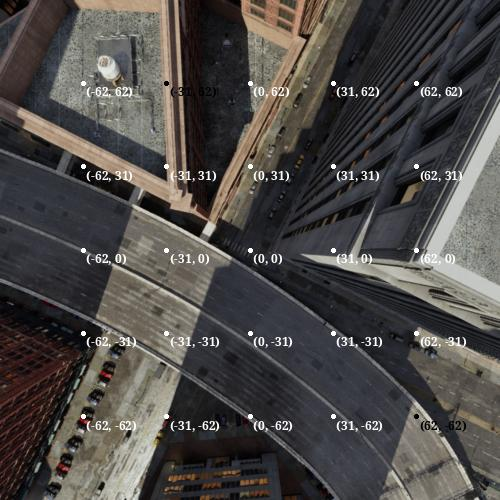
\includegraphics[width=0.5\linewidth]{images/GPT4o-CityNew/21_r0__0.jpg}
    \end{center}
    
\respeaks: Your current altitude is 93 meters above ground level.
\gptspeaks: \( < \)Reasoning\( > \)The black truck might be under the overpass or in the parking areas at the bottom. I'll move southwest toward the (-62, -31) position and decrease altitude to get a better view.\( < \)/Reasoning\( > \)
\( < \)Action\( > \)(-62, -31, -20)\( < \)/Action\( > \)
\respeaks: Emergency stop; you've flown too close to something and would have hit it.
\StageDir{\re{} presents \gpt{} with a relevant image}

    \begin{center}
    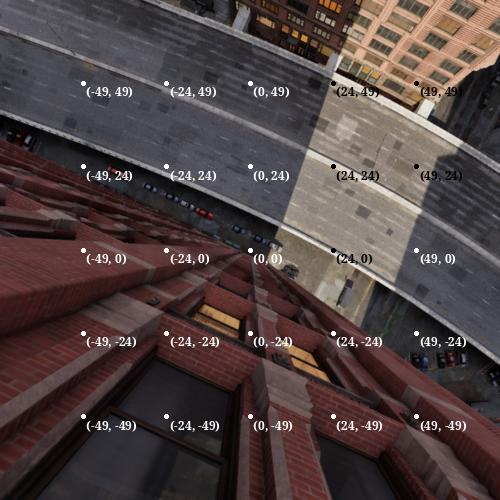
\includegraphics[width=0.5\linewidth]{images/GPT4o-CityNew/21_r0__1.jpg}
    \end{center}
    
\respeaks: Your current altitude is 73 meters above ground level.
\gptspeaks: \( < \)Reasoning\( > \)I'll proceed more carefully and move slightly east toward the (-24, 0) position to inspect the parking area, while maintaining a safe altitude adjustment.\( < \)/Reasoning\( > \)
\( < \)Action\( > \)(-24, 0, -10)\( < \)/Action\( > \)
\respeaks: Emergency stop; you've flown too close to something and would have hit it.
\StageDir{\re{} presents \gpt{} with a relevant image}

    \begin{center}
    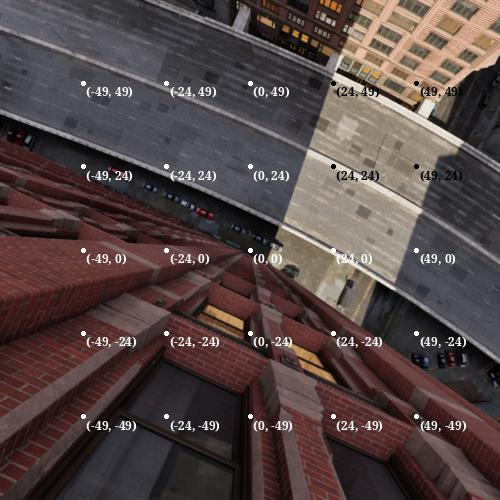
\includegraphics[width=0.5\linewidth]{images/GPT4o-CityNew/21_r0__2.jpg}
    \end{center}
    
\respeaks: Your current altitude is 73 meters above ground level.
\gptspeaks: \( < \)Reasoning\( > \)I'll adjust my approach and move east toward the (0, 24) position, keeping a higher altitude to avoid obstacles.\( < \)/Reasoning\( > \)
\( < \)Action\( > \)(0, 24, 0)\( < \)/Action\( > \)
\StageDir{\re{} presents \gpt{} with a relevant image}

    \begin{center}
    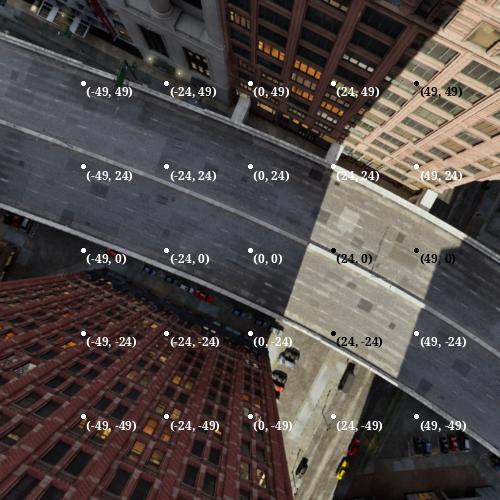
\includegraphics[width=0.5\linewidth]{images/GPT4o-CityNew/21_r0__3.jpg}
    \end{center}
    
\respeaks: Your current altitude is 73 meters above ground level.
\gptspeaks: \( < \)Reasoning\( > \)The black truck might be in the parking area below. I'll move southeast toward the (24, -24) position and decrease the altitude for a closer look.\( < \)/Reasoning\( > \)
\( < \)Action\( > \)(24, -24, -20)\( < \)/Action\( > \)
\StageDir{\re{} presents \gpt{} with a relevant image}

    \begin{center}
    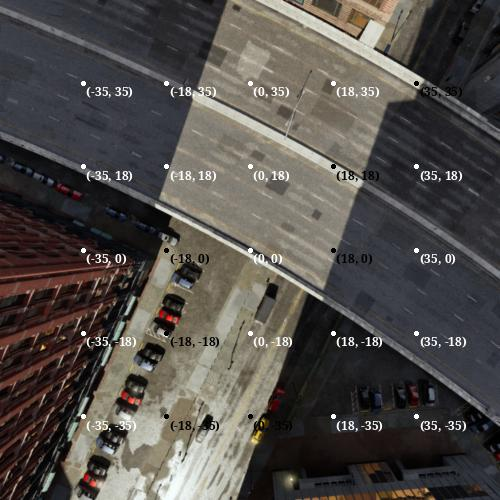
\includegraphics[width=0.5\linewidth]{images/GPT4o-CityNew/21_r0__4.jpg}
    \end{center}
    
\respeaks: Your current altitude is 53 meters above ground level.
\gptspeaks: \( < \)Reasoning\( > \)The black truck might be in the parking area to the southwest. I'll move to the (-18, -18) position and decrease altitude to get a closer view.\( < \)/Reasoning\( > \)
\( < \)Action\( > \)(-18, -18, -20)\( < \)/Action\( > \)
\StageDir{\re{} presents \gpt{} with a relevant image}

    \begin{center}
    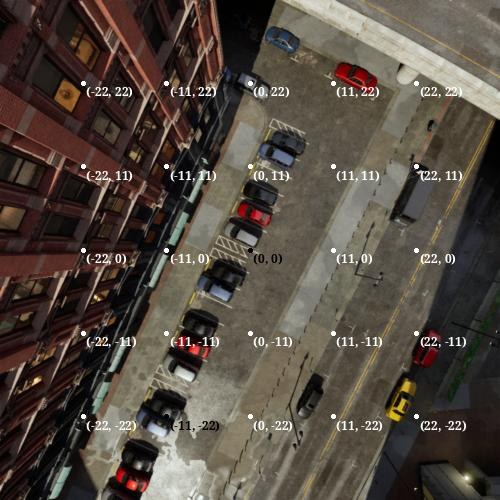
\includegraphics[width=0.5\linewidth]{images/GPT4o-CityNew/21_r0__5.jpg}
    \end{center}
    
\respeaks: Your current altitude is 33 meters above ground level.
\gptspeaks: \( < \)Reasoning\( > \)A black truck is visible at the (0, 22) position. I'll move there and decrease altitude to ensure I'm within 10 meters above it.\( < \)/Reasoning\( > \)
\( < \)Action\( > \)(0, 22, -25)\( < \)/Action\( > \)
\StageDir{\re{} presents \gpt{} with a relevant image}

    \begin{center}
    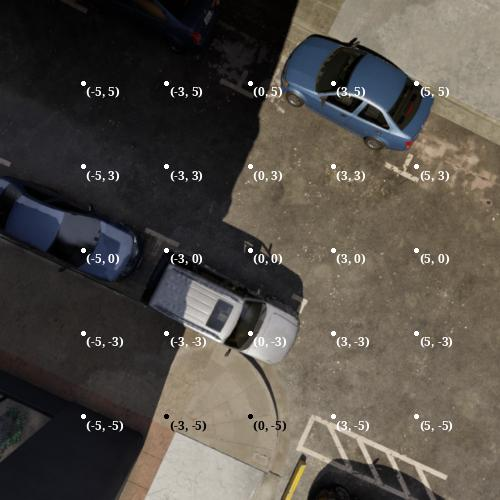
\includegraphics[width=0.5\linewidth]{images/GPT4o-CityNew/21_r0__6.jpg}
    \end{center}
    
\respeaks: Your current altitude is 8 meters above ground level.
\gptspeaks: \( < \)Reasoning\( > \)I am now centered above the black truck and within 10 meters of altitude. The truck is clearly visible.\( < \)/Reasoning\( > \)
\( < \)Decision\( > \)FOUND\( < \)/Decision\( > \)
\end{drama}
\subsubsection{Example}

    \begin{itemize}[noitemsep,topsep=0pt]
      \item Starting position: (0.0, -3.0, 69.0)
      \item End position: (0.0, -67.0, 9.0) 
      \item Euclidean distance from the object: 67.60177512462228
      \item Object can be seen: False
      \item Success: False
      \item Object type: a fire
      
    \end{itemize}
    

    \begin{center}
    \includegraphics[width=0.7\linewidth]{images/GPT4o-CityNew/22_r0_.pdf}
    \end{center}
    

    \begin{center}
    \includegraphics[width=0.7\linewidth]{images/GPT4o-CityNew/22_r0__sit_awareness.pdf}
    \end{center}
    

    \begin{drama}
    \Character{Benchmark}{re}
    \Character{GPT-4o}{gpt}
    
\respeaks: \( < \)Context\( > \)
    You are in command of a UAV, tasked with finding a fire.
\( < \)/Context\( > \) \texttt{(REST OF THE PROMPT)}
\StageDir{\re{} presents \gpt{} with a relevant image}

    \begin{center}
    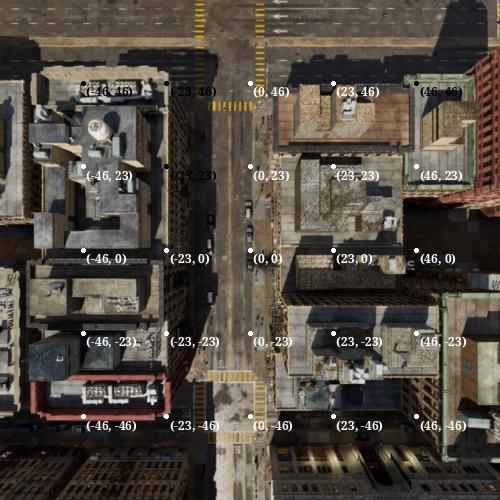
\includegraphics[width=0.5\linewidth]{images/GPT4o-CityNew/22_r0__0.jpg}
    \end{center}
    
\respeaks: Your current altitude is 69 meters above ground level.
\gptspeaks: \( < \)Reasoning\( > \)There is no visible fire in the current image. I will move north to get a better view of more rooftops. I will also lower the altitude to get a closer look.\( < \)/Reasoning\( > \)
\( < \)Action\( > \)(0, 46, -20)\( < \)/Action\( > \)
\StageDir{\re{} presents \gpt{} with a relevant image}

    \begin{center}
    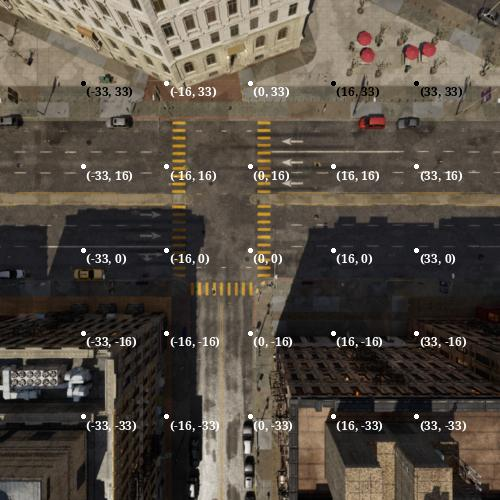
\includegraphics[width=0.5\linewidth]{images/GPT4o-CityNew/22_r0__1.jpg}
    \end{center}
    
\respeaks: Your current altitude is 49 meters above ground level.
\gptspeaks: \( < \)Reasoning\( > \)Still no visible fire in the current image. I will move further north and decrease altitude to continue the search.\( < \)/Reasoning\( > \)
\( < \)Action\( > \)(0, 33, -20)\( < \)/Action\( > \)
\StageDir{\re{} presents \gpt{} with a relevant image}

    \begin{center}
    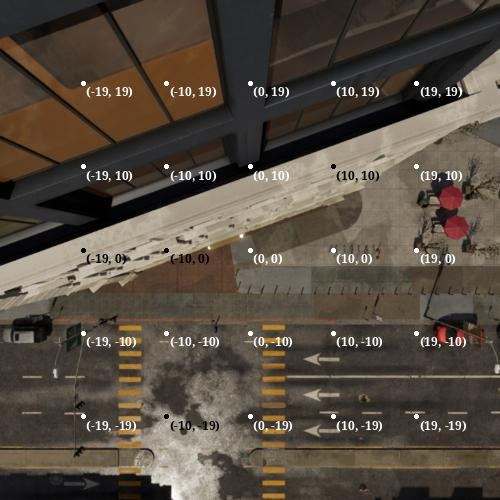
\includegraphics[width=0.5\linewidth]{images/GPT4o-CityNew/22_r0__2.jpg}
    \end{center}
    
\respeaks: Your current altitude is 29 meters above ground level.
\gptspeaks: \( < \)Reasoning\( > \)I can see smoke coming from the street area. I will move slightly south and lower the altitude to get closer to the possible source of the fire.\( < \)/Reasoning\( > \)
\( < \)Action\( > \)(0, -10, -15)\( < \)/Action\( > \)
\StageDir{\re{} presents \gpt{} with a relevant image}

    \begin{center}
    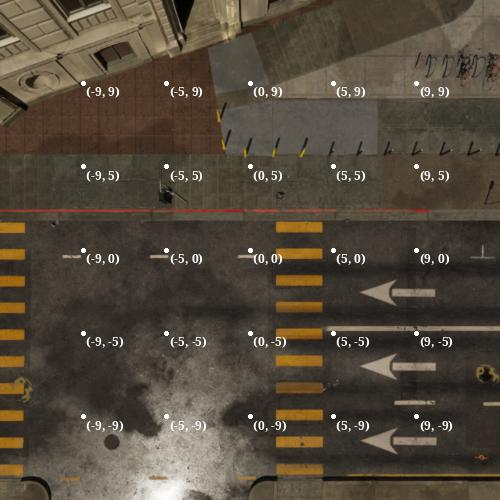
\includegraphics[width=0.5\linewidth]{images/GPT4o-CityNew/22_r0__3.jpg}
    \end{center}
    
\respeaks: Your current altitude is 14 meters above ground level.
\gptspeaks: \( < \)Reasoning\( > \)The fire is now clearly visible in the bottom center of the image. I will lower the altitude slightly to be within 10 meters above the fire.\( < \)/Reasoning\( > \)
\( < \)Action\( > \)(0, -5, -5)\( < \)/Action\( > \)
\StageDir{\re{} presents \gpt{} with a relevant image}

    \begin{center}
    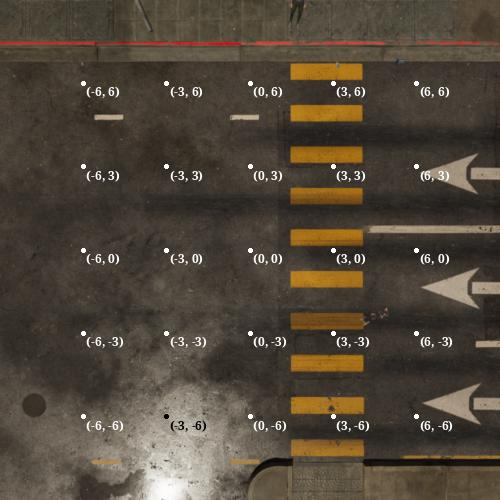
\includegraphics[width=0.5\linewidth]{images/GPT4o-CityNew/22_r0__4.jpg}
    \end{center}
    
\respeaks: Your current altitude is 9 meters above ground level.
\gptspeaks: FOUND
\end{drama}
